For small-scale systems, we have discussed the Hartree-Fock
and Density Functional Theory methods as the primary workhorses of ab-initio
electronic structure calculations. However, these methods suffer
from very poor scaling as the system size increases, with Hartree-Fock
naively scaling as $\mathcal{O}(N^4)$ with $N$ the number of electrons
and Density Functional Theory scaling as $\mathcal{O}(N^4)$,
but with a larger proportionality scaling.
In many cases the exact details of the electronic structure
are less important than the long-time behaviour of the atoms
and molecules involved in the simulation, and classical approximations
can be made as in molecular dynamics, which comes close
to linear scaling. This allows us to simulate systems
of up to millions or hundreds of millions of atoms,
which can approximate nano- or micro-scale systems if
periodic boundary conditions are applied.
However, the question remains as to how you develop an
accurate classical potential which can accurately reproduce
fundamentally quantum systems, with a speed that allows
us to enter into realistic timescales (i.e. nano or microseconds).
\par
The most common approach to developing molecular dynamics potentials
is to guess a functional form based on your physical intuition
and experience with the systems and calculate appropriate parameters
from data obtained from DFT calculations.
The number of parameters involved can range from two in the case
of Lennard-Jones or hundreds of parameters in the case
of complex, many-atom potentials such as the AMBER and CHARMM
force fields. The imposition of functional forms to quantum data
is an artform, and the potential must often be tailored to not
only the chemical species and number of atoms in your system,
but also the specific experimental quantity you are trying to extract,
such as the energy, radial distribution function or transport
coefficients. Notably there are dozens of MD potentials
describing different models of water (H2O), each fine-tuned
for a specific system structure or parameter.
\newline
\newline
Due to recent developments in the field of machine learning,
the question has been raised as to how it may be possible to
automate the process of developing potentials.
In their article introducing the Atomistic Machine-Learning Package
(AMP) \parencite[Khorshidi, Alireza and Peterson, Andrew A.]
{khorshidi2016amp} outline one potential way forward.
The idea is to approximate the potential energy
with a regression model:

\begin{equation}
 \left\{ \bm{R} \right\} \overset{\text{Regression}}{\longrightarrow}
    E = E\left( \left\{ \bm{R} \right\}\right) , 
\end{equation}

where $\left\{\bm{R}\right\}$ is the set of nuclear coordinates of our system.
Most machine learning methods operate over a set of one-dimensional
so-called \textit{feature vectors}, where every vector element
represents a feature of the data set. For example the amount
of precipation in a given area at a given time is a function
of features such as humidity, cloud cover, air pressure etc.
This is a vector of some length $D$, while the nuclear coordinates
represent a point in $3N$-dimensional phase space.
This difference in representation requires some way of mapping
the nuclear coordinates to features which can be employed
by a machine learning method.
The naive approach would be to simply feed in the nuclear coordinates
as a 1D vector, and then perform a regression on the dataset
in order to obtain the potential energy. However, our physical intuition
imposes some constraints on the potential energy.
In particular, the potential energy of a microscopic system should
be translationally, rotationally and permutationally invariant.
\par
Translational invariance implies that the addition of any
three-dimensional vector to every coordinate in the system should
not in any way alter the potential energy of the system.
This should not be the case with a naive mapping, as for a given
set of weights (or equivalent) smaller/larger coordinates
values would be mapped to smaller/larger activations, and therefore
alter the final output.
Rotational invariance implies that the potential energy
of the system should not change as the system is rotated
about an axis. This also should not be the case in the context
of a naive mapping, as any change to any of the inputs
would be mapped in a non-linear way to produce a different output.
Finally, permutation invariance implies that swapping the coordinates
of any two atoms of the same chemical species would produce the
same potential energy. This should also not be the case, for
the same reasons as we just discussed.
These constraints together heavily restrict the functional form
that any mapping to the potential energy could have,
which means a more careful analysis should be considered.
\newline
\newline
In order for the mapping to be applicable to systems of varying size,
a decomposition into atomic energy contributions is performed:

\begin{equation}
 E(\left\{\bm{R}\right\}) = \sum_{i=1}^N E_{\text{atom}}
 (\left\{\bm{R}\right\}) . 
\end{equation}

The individual energy contributions $E_{\text{atom}}$
are then approximated by performing a regression analysis.
The atomic energy contributions are usually limited to its
local environment through the introduction of a cutoff radius $R_c$:

\begin{equation}
 E_{\text{atom}} (\left\{\bm{R}\right\}) \approx
    E_{\text{atom}} (\bm{R}_i, \left\{\bm{R}\right\}_j 
    | \left| \bm{R}_{ij} \right|
    < R_c) 
\end{equation}

meaning that interactions are only treated if the interatomic distance
is smaller than the cutoff. This is a good approximation for a sensible
choice of cutoff radius if no electrostatic interactions are involved.
Long-range interactions can also be treated through
the introduction of methods such as Ewald summation, but this will
not be discussed here.
A mapping that satisfies the above constraints we will refer to
as a \textit{descriptor}, and is used as input to the regression method:

\begin{equation}
    \left\{\bm{R}\right\} \rightarrow \bm{G}(\left\{\bm{R}\right\}) 
    \overset{\text{regression}}
    {\longrightarrow} E_{\text{atom}} =
    E_{\text{atom}}(\bm{G}(\left\{\bm{R}\right\})). 
\end{equation}

Once we have a descriptor and a regression model the dynamics
can be readily obtained by taking derivatives. The force on atom
$i$ is calculated as:

\begin{equation}
\begin{split}
    \bm{F}_i &= -\nabla_i E \\
    &= -\nabla_i \sum_i^{\text{local}}
    E_{\text{atom}}(\bm{G}(\left\{\bm{R}\right\})) \\
    &= -\sum_i^{\text{local}} \sum_j \frac{\partial E_{\text{atom}}}
    {\partial G_j} \frac{\partial G_j}{\partial \bm{R}_i} ,
\end{split}
\end{equation}

where we have applied the chain rule to break the gradient
into derivatives with respect to the network inputs (obtained through
backpropagation) and derivatives of the network inputs with
respect to the coordinates of atom $i$.
Once we have obtained the forces the system can be propagated through time
classically using for example the Velocity-Verlet equations (see for
example \cite{martys1999velocity}).

\subsection{Gaussian descriptors}\label{chap:gaussian}
In their paper on neural-network representations of
potential energy surfaces \parencite[Behler, J\"{o}rg and
Parrinello, Michele]{behler2007generalized}
suggested the decomposition of the mapping $\bm{G}_i$ of atom $i$
into two subvectors $\bm{G}_i^I$ and $\bm{G}_i^{II}$ representing
pairwise and three-body interactions respectively.
The components of $\bm{G}_i^I$ are comprised of
sums of gaussian functions of the pairwise distance $R_{ij}$:

\begin{equation}
 f_i^I = \sum_{j \neq i}^{\text{local}}
    \exp \left( -\eta(R_{ij} - R_s)^2 / R_c^2 \right) f_c (R_{ij}) , 
\end{equation}

with the sum over the local environment of atom $i$.
This form of the radial symmetry functions is known as the G2 type,
while other forms are possible such as the G1 type which sums over
cutoff functions only.
The parameters $\eta$ and $R_s$ represent the width and center
of the gaussian functions respectively. The term $f_c$
is a cutoff function which decays smoothly to zero
at the cutoff radius. Behler and Parrinello proposed
the following cutoff:

\begin{equation}
    f_c(R) =
\begin{cases}
    \frac{1}{2}\left(1 + \cos \left(\pi R / R_c \right) \right) & R < R_c \\
    0 & R \geq R_c ,
\end{cases}
\end{equation}

however other functional forms are possible.
The only requirements we pose
is that the function be continuous with a continuous first derivative
in $r \in [0, \infty)$,
approach one as $R \rightarrow 0$
and zero as $R \rightarrow R_c$.
The AMP authors propose an alternative polynomial cutoff function:

\begin{equation}
    f_c(R) =
\begin{cases}
    1 + \gamma \cdot (r / R_c)^{\gamma + 1} - (\gamma + 1)(r / R_c)^{\gamma} & R < R_c \\
    0 & R \geq R_c ,
\end{cases}
\end{equation}

where $\gamma$ is a user-specified parameters that controls the rate of decay.
For values of $\gamma < 2$ this cutoff reproduces the cosine cutoff, while for higher
values the polynomial has much larger values within the cutoff radius.
Figure \ref{fig:cutoff} shows the cutoff functions plotted together
for different values of $\gamma$.
Figure \ref{fig:symmetry-functions} shows radial and angular parts of the symmetry functions
with different parameter values, where the radial functions are centered at $R_s = 0$.

\begin{figure}[H]
    \centering
    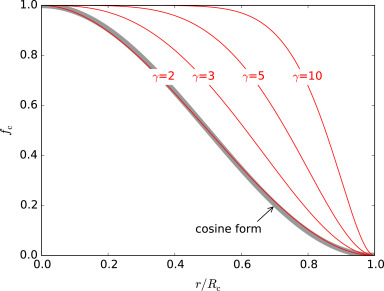
\includegraphics[width=0.7\textwidth]{cutoff.jpg}
    \caption{Cosine and polynomial cutoff functions plotted within
        the cutoff radius. 
        The polynomial cutoff reproduces the cosine cutoff for small values
        of $\gamma$.
        Reprinted from \parencite[
            Khorshidi, Alireza and Peterson, Andrew A.]{khorshidi2016amp}.}
    \label{fig:cutoff}
\end{figure}

\begin{figure}[H]
    \centering
    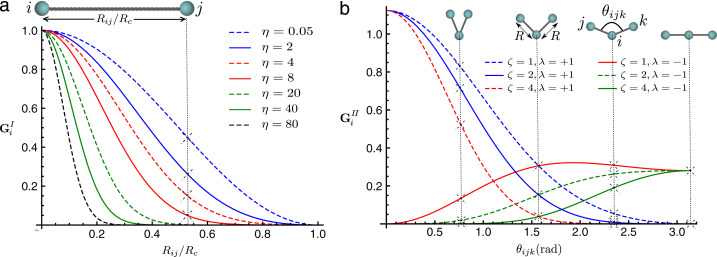
\includegraphics[width=\textwidth]{symmetry_functions.jpg}
    \caption{Radial and angular symmetry functions for different values
        of $\eta, \zeta, \lambda$. The radial symmetry functions
        are centered at $R_s = 0$. Reprinted from \parencite[
            Khorshidi, Alireza and Peterson, Andrew A.]{khorshidi2016amp}.}
    \label{fig:symmetry-functions}
\end{figure}

The components of the three-body subvector are defined incorporating
the angles $\theta_{ijk}$ between every triplet of atoms:

\begin{equation}
\begin{split}
    f_i^{II} &= 2^{1 - \zeta} \sum_{j,k \neq i}^{\text{local}}
    (1 + \lambda \cos \theta_{ijk})^{\zeta}
    \exp \left( -\eta \left( R_{ij}^2 + R_{ik}^2 + R_{jk}^2
    \right) / R_c^2 \right) \\
    & \times f_c(R_{ij}) f_c(R_{ik}) f_c(R_{jk}) .
\end{split}
\end{equation}

This form of angular function is known as the G5 type, while the G4
angular symmetry functions do not contain the $R_{jk}$ terms.
The components for each subvector is calculated by varying
the different parameters $\eta, R_s, \zeta, \lambda$.
The choice of neither symmetry functions, cutoff, nor the parameters
employed by Behler and Parrinello are unique. The guiding
wisdom is that atomic environments with different
potential energies should give differing energies,
while remaining invariant under translation, rotation and permutation.
Finally we note that the descriptors and the neural network
models are not interchangeable, as each neural network
is trained for a specific set of input vectors, and must
be retrained if the way inputs are composed changes.

\subsection{Zernike and bispectrum descriptors}
Two closely related examples of atom-centered descriptors
are the Zernike and Bispectrum descriptors.
They are described by \parencite[Khorshidi, Alireza and Peterson,
Andrew A.]{khorshidi2016amp} in their paper
on the Atomistic Machine-learning Package (AMP).
Bispectrum descriptors are also discussed by
\parencite[Behler, J\"{o}rg]{behler2016perspective}
in his perspective on machine learning potentials.
Zernike descriptors represent a tensor product between spherical
harmonics and Zernike polynomials. The local atomic environment
of atom $i$ is represented by an atomic density function $\rho_i(\bm{r}_i)$:

\begin{equation}
 \rho_i(\bm{r}_i) = \sum_{j\neq i}^{\text{local}}
    \eta_j \delta \left( \bm{r}_i - \bm{r}_{ij} \right)
    f_c \left( \lvert \lvert \bm{r}_{ij} \rvert \rvert \right) , 
\end{equation}

with $f_c(r)$ a cutoff function as described in the previous section.
The 3-D Zernike basis set $Z$ is formed by a tensor product between
the Zernike polynomials basis set $R$ and the spherical harmonics
$Y$. The Zernike basis set is defined inside and on the surface
of the $S^2$ unit sphere as:

\begin{equation}
 Z_{nl}^m (r, \theta, \phi) = R_n^l(r) Y_l^m(\theta, \phi) , 
\end{equation}

where $n \geq 0$ is an integer, $l$ is restricted to even $n - l \geq 0$
and $m$ is an integer such that $\left| m \right| \leq l$.
Functions defined inside and on the $S^2$ sphere
can be represented by the 3-D Zernike basis as:

\begin{equation}
 f(r, \theta, \phi) = \sum_{n=0}^{\infty} \sum_l \sum_{m=-l}^l
    c_{nl}^m Z_{nl}^m (r, \theta, \phi) , 
\end{equation}

with coefficients $c_{nl}^m = \langle Z_{nl}^m, f \rangle$
computed as projections of $f$ onto the Zernike basis.
These projections form the basis of the Zernike fingerprint,
$\bm{G}_i$. Centering the atomic density preserves translation
invariance of the atomic environment, while the projections
onto the Zernike basis set preserves rotational invariance.
Permutation invariance is maintained by keeping the constant values
$\eta_j$ the same within each chemical species.
The Zernike descriptors are able to incorporate quadruple
atomic interactions involving for example dihedral angles,
while the gaussian descriptors are truncated at threebody
interactions. The Zernike coefficients can also often be represented
in terms of monomials, making them computationally cheaper
than the bispectrum descriptors.
\par
Bispectrum descriptors are computed much in the same way
as the Zernike descriptors. The 4-D spherical harmonics
form a complete, orthogonal basis set for the $S^3$ 4-D unit
sphere, and the components of the Bispectrum fingerprints
$\bm{G}_i$ can be computed by projecting the atomic
density function onto them. For more information
the reader is encouraged to check out the \parencite[AMP paper]
{khorshidi2016amp}.

\subsection{Deep Potential Molecular Dynamics}
Deep Potential Molecular Dynamics (DPMD) is a method
proposed by \parencite[Zhang et al.]{PhysRevLett.120.143001}
in response to the successes of methods such as Behler-Parrinello,
Gaussian Approximation Potentials (GAP\cite{PhysRevLett.104.136403})
and Gradient-Domain Machine Learning (GDML\cite{Chmielae1603015}).
These methods all involve some amount of handcrafting the inputs,
and building these inputs for larger, more complex systems is not
always straightforward.
The Deep Potential method assigns a local environment and reference
frame to each atom. The total potential energy is a sum
of atomic contributions as before:

\begin{equation}
 E = \sum_i E_{\text{atom}}\left( \left\{ \bm{R} \right\} \right),
\end{equation}

with the atomic energy determined by its nearest neighbors
within a cutoff radius $R_c$:

\begin{equation}
    E_{\text{atom},i} = E\left(\bm{R}_i,
    \left\{ \bm{R} \right\}_j : \left| \bm{R}_{ij}
    \right| < R_c \right) . 
\end{equation}

The position of each neighbor of atom $i$ is described
by the relative position $\bm{R}_{ij} = \bm{R}_j - \bm{R}_i$,
which preserves translational symmetry.
Rotational symmetry is conserved by constructing a local frame
for each atom. Two neighboring atoms $a$ and $b$ are picked by a
user-specified rule (default: two closest).
The environment of atom $i$ is then described by three unit vectors:

\begin{equation}
\begin{split}
    \bm{e}_{i1} &= \bm{e}(\bm{R}_{ia}) , \\
    \bm{e}_{i2} &= \bm{e}(\bm{R}_{ib} - (\bm{R}_{ib} \cdot \bm{e}_{i1})
    \bm{e}_{i1}) , \\
    \bm{e}_{i3} &= \bm{e}_{i1} \times \bm{e}_{i2} ,
\end{split}
\end{equation}

where $\bm{e}(\bm{R})$ denotes the normalized vector $\bm{e}(\bm{R})
    = \bm{R} / \left| \bm{R} \right|$. Together these vectors
form an orthonormal basis for the reference frame of atom $i$.
The local coordinates $\bm{R}_{ij}$
can then be obtained from the global coordinates $\bm{R}_{ij}^0$
through the transformation:

\begin{equation}
    \bm{R}_{ij} = \bm{R}_{ij}^0 \cdot \mathcal{R} ,
\end{equation}

where $\mathcal{R} = [\bm{e}_{i1} \ \bm{e}_{i2} \ \bm{e}_{i3}]$
is a rotation matrix with columns given by the local basis vectors.
The neural network input vector for every atom-to-atom interaction
$\bm{D}_{ij}$ can be given with radial-only or full radial-angular
information:

\begin{equation}
    \bm{D}_{ij}^{\alpha} =
\begin{cases}
    \displaystyle\left( \frac{1}{R_{ij}}, \frac{\bm{R}_{ij}}{\left| \bm{R}_{ij} \right|}
    \right) & \text{full information}, \\[10pt]
    \displaystyle\left( \frac{1}{R_{ij}} \right) & \text{radial-only information},
\end{cases}
\end{equation}

with $\alpha = 0$ when only radial information is specified
and $\alpha = 0,1,2,3$ when full information is provided. Radial information
is typically sufficient for long-range interactions such as van-der-Waals
forces, while covalent bonding can be modeled by including
only the closest atoms. We therefore specify two separate
cutoff shells, one for the radial information $R_c$ and one
for treating angular interactions $R_a$.
\par
In order to preserve permutation symmetry the input vectors $\bm{D}_{ij}$
are sorted first according to chemical species, and then within
each chemical species according to their inverse distance $1 / R_{ij}$.
The vector of subvectors $\bm{D}_i$ is then fed through a neural
network to produce the atomic energy contribution.
The network input size is fixed according to the maximum number of neighbors
in the system which is being studied, with some entries $\bm{D}_{ij} = \bm{0}$
if there are fewer neighbors within the radial cutoff.
Figure \ref{fig:dpmd} shows how the neural network input vector
is computed for the environment of a hydrogen atom.

\begin{figure}[H]
    \centering
    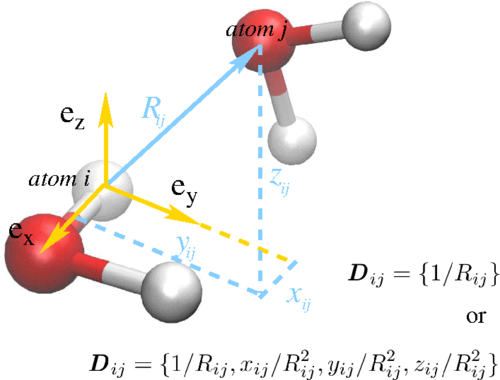
\includegraphics[width=\textwidth]{dpmd.png}
    \caption{Computation of the neural network input vector for atom $i$.
        Hydrogen in white and oxygen in red.
        The coordinates of atom $j$ are computed in the 
        reference system of atom $i$.
        The vector $\bm{e}_x$ is along the OH bond, $\bm{e}_y$ is perpendicular
        to the plane of the water molecule and $\bm{e}_z$ is the cross product.
        The subvector $\bm{D}_{ij}$ forms part of the input vector
        $\bm{D}_i$ computed from the atom's nearest neighbors.
        The vector $\bm{D}_i$ is fed through a neural network
        to produce an atomic potential energy contribution.
        Reprinted from \parencite[Zhang et al.]{PhysRevLett.120.143001}.}
    \label{fig:dpmd}
\end{figure}

The authors also propose a scheme of force learning, wherein
the force root mean square error (RMSE) is incorporated into the Cost function:

\begin{equation}
    \mathcal{C} = \frac{p_{\epsilon}}{N} \sum_i
    \left( \Delta E_i^2 \right)
    + \frac{p_{f}}{3N} \sum_i \left| \Delta \bm{F}_i \right|^2,
\end{equation}

with $p_{\epsilon}$ and $p_{f}$ energy and force pre-factors which are
adjusted throughout the learning process. The term $\Delta E_i$
denotes the error between the network outputs
and the correct potential energy, while the term $\Delta \bm{F}_i$
denotes the error in the force output.
The pre-factors are adjusted based on the learning rate:

\begin{equation}
    p(t) = p^{\text{limit}} \left[ 1 - \frac{r_l(t)}{r_l^0} \right]
    + p^{\text{start}} \left[ \frac{r_l(t)}{r_l^0} \right] ,
\end{equation}

with $r_l(t)$ and $r_l^0$ the learning rate at time step $t$ and time step
$0$ respectively. The learning rate decays exponentially as:

\begin{equation}
 r_l(t) = r_l^0 \cdot d_{r}^{\left(t / d_s\right)} , 
\end{equation}

with $d_r$ the decay rate and $d_s$ the decay steps. The decay
rate should be less than 1. The force error is often a magnitude or two
larger than the energy error, and it is believed that incorporating
the force into the loss should improve the learning rate for
physics-based applications which incorporate forces.
The virial information can also be treated in this manner,
but we will not discuss this here.
